\subsection{Visualizzazione dataset salvati}

\begin{figure}[H]
    \centering
    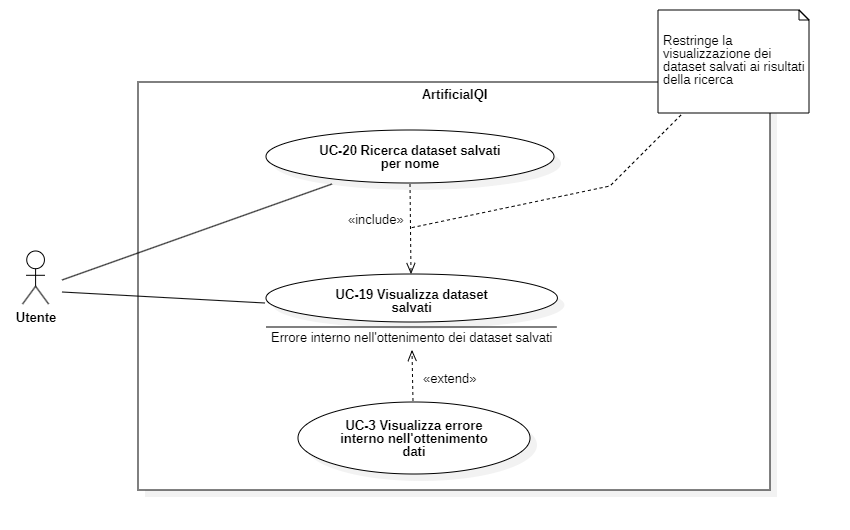
\includegraphics[scale=0.23]{Sezioni/UseCase/Immagini/VisualizzazioneDatasetSalvati}
    \caption{Diagramma visualizzazione dataset salvati.}
\end{figure}

\begin{usecase}{UC-22}{Visualizza dataset salvati}
    \label{uc:UC-22}
    
    \req{\hyperref[ru:RUO-3]{RUO-3}} 

    \pre{}

    \post{
        \item L'utente visualizza i dataset salvati
    }
    
    \actor{Utente}

    \trigger{L'utente vuole visualizzare i dataset salvati}

    \inc{}

    \base{}

    \scenario{
        \item L'utente richiede di visualizzare i dataset salvati
        \item Il sistema ottiene i dataset salvati
        \item Il sistema verifica la presenza di dataset salvati
        \item Vengono visualizzata la lista dei dataset salvati
    }

    \subscenario{
        \item[2.1] Il sistema verifica un errore interno durante l'ottenimento dei dataset salvati:
        \begin{itemize}
            \item \hyperref[uc:UC-3]{UC-3}
        \end{itemize}
        \item[3.1] Non esistono dataset salvati:
        \begin{itemize}
            \item Viene notificato all'utente che non esistono dataset salvati
        \end{itemize}
    }
\end{usecase}


\begin{usecase}{UC-23}{Ricerca dataset salvati per nome}
    \label{uc:UC-23}
    
    \req{\hyperref[ru:RUO-4]{RUO-4}} 

    \pre{
        \item L'utente sta visualizzando i dataset salvati
    }

    \post{
        \item L'utente visualizza la lista dei dataset salvati che contengono nel nome le parole chiave indicate
    }
    
    \actor{Utente}

    \trigger{}

    \inc{\hyperref[uc:UC-22]{UC-22}}

    \base{}

    \scenario{
        \item L'utente specifica le parole chiave da utilizzare nella ricerca
        \item L'utente richiede l'esecuzione della ricerca
        \item Il sistema seleziona l'insieme di dataset salvati che contengono le parole chiave nel nome
        \item Il sistema mostra il precedente insieme seguendo \hyperref[uc:UC-22]{UC-22}
    }
    \subscenario{}
\end{usecase}
